Avant même d'aborder les fonctionalités graphiques de R, nous devons préciser qu'elles sont quasi infinies. C'est donc pour cette raison que nous nous contenterons de survoler les types de graphiques qui combleront amplement vos besoins pour faire vos premiers pas. Advenant le cas où ces connaissances ne seront plus suffisantes, il existe énormément d'exemples sur les forums de la communauté pour apaiser votre curiosité. \\

Pour débuter, la fonction \texttt{plot} \cite{Rfunction:plot} est de loin la fonction graphique la plus générique en R. Cette fonction ne possède que trois arguments: \texttt{x}, \texttt{y} et \texttt{...}. Naturellement, nous devrons fournir des valeurs d'abscisse et d'ordonnée à la commande \texttt{plot} via les arguments \texttt{x} et \texttt{y}. Par la suite, la fonction s'occupera de produire un nuage de points . En partant directement du jeu de données \texttt{airports.dat}, nous pouvons être tentés d'essayer cette commande en représentant les couples longitude/latitude de chaque aéroport dans le monde. Bien entendu, le résultat obtenu sera peu élégant ne représentant que l'essentiel. \\

C'est à ce moment que l'argument \texttt{...} entre en scène. Nous n'avons pas discuté de ce type d'argument dans la section précédente puisque nous considérions plus intuitif de le présenter à l'aide de son utilisation la plus commune, soit le passage d'options graphiques au sein de la commande \texttt{plot}. Il ne sera toutefois pas rare de retrouver cet argument dans bon nombre de fonctions, mais sa nécessité sera souvent moindre que dans le cas de la création de graphiques. Cet argument possède la propriété particulière d'absorber tous les paramètres qui seront passés à la fonction et qui n'auront pas été assignés à un argument. Ces mêmes paramètres pourront donc ensuite être transmis à une autre fonction dans le corps de la fonction. \\

C'est exactement ce qui se produit dans le cas de la commande \texttt{plot} qui enverra tous les paramètres supplémentaires à la fonction \texttt{par} \cite{Rfunction:par} (la commande gérant tous les aspects des graphiques en R). Heureusement, il existera des comportements par défaut pour tous les arguments de cette fonction. Il sera inconcevable et surtout inutile à quiconque d'apprendre l'ordre réel dans lequel ses arguments se présentent. Le passage des paramètres se fera donc en nommant chaque argument sur lequel nous voulons imposer un comportement différent. \\

\begin{moreInfo}{\texttt{par} magie!}
	La fonction \texttt{par} vous sera de grands secours à plusieurs reprises. Une utilisation fréquente et explicite de cette fonction est de modifier la division de la fenêtre d'affichage de R. En modifiant la valeur de l'argument \texttt{mfrow}, nous pourrons ainsi combiner plusieurs graphiques intimement reliés sur la même fenêtre graphique facilitant du même coup leur comparaison. \\
	Par exemple, \texttt{par(mfrow = c(2,2))} divisera la fenêtre en 2 lignes et 2 colonnes pour ainsi accueillir 4 graphiques distincts.
\end{moreInfo}

C'est précisément ce que nous avons fait dans la deuxième version de notre graphique (\autoref{fig:LonLatMap}) en spécifiant le nom des axes (\texttt{xlab} et \texttt{ylab}) ainsi qu'un titre au graphique (\texttt{main}). Nous avons aussi modifié le type de point pour passer de points vides à des points remplis (\texttt{pch}) tout en réduisant la taille de ces derniers pour obtenir une meilleure résolution (\texttt{cex}). Finalement, nous avons utilisé une police en gras pour le titre du graphique et les axes (\texttt{font} et \texttt{font.lab}) en plus de venir augmenter la taille de ces derniers (\texttt{cex.main} et \texttt{cex.lab}). Référez-vous au \autoref{src:plot} pour plus de précisions. \\
	
\begin{figure}
	\begin{minipage}{\textwidth}
		\centering
		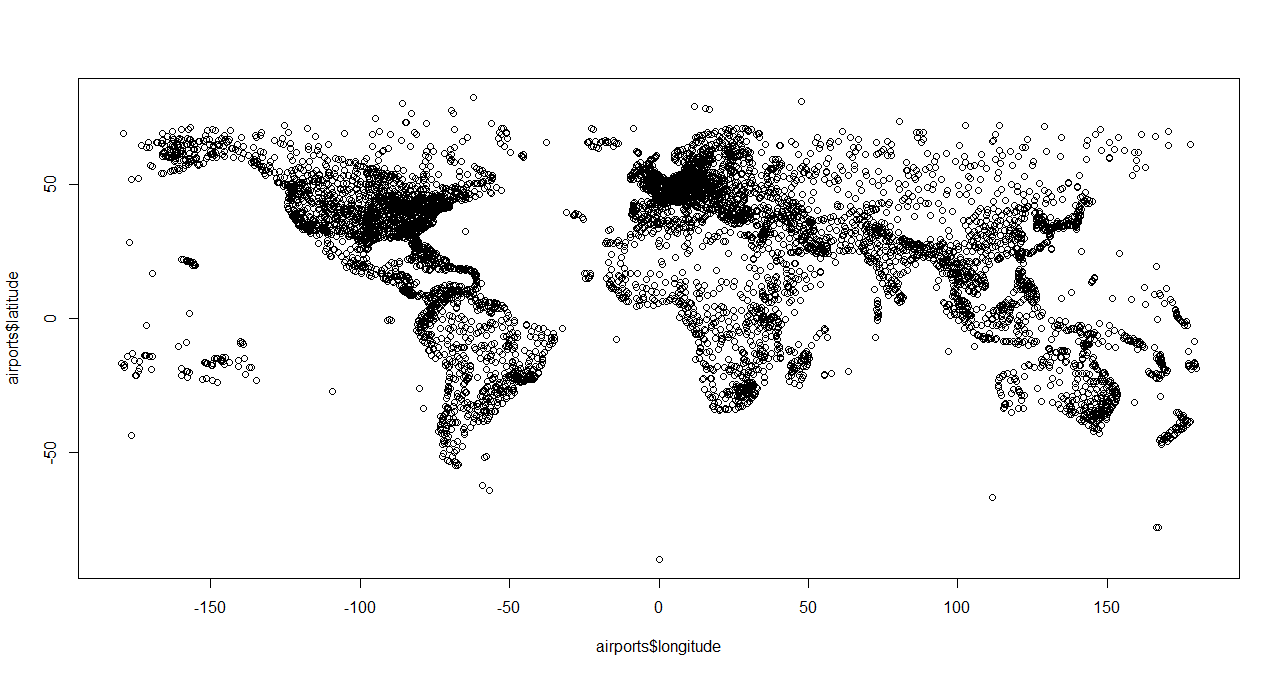
\includegraphics[width=\textwidth, height=\textheight,keepaspectratio]{LonLatMapV1}
	\end{minipage}
	\newline
	\begin{minipage}{\textwidth}
		\centering
		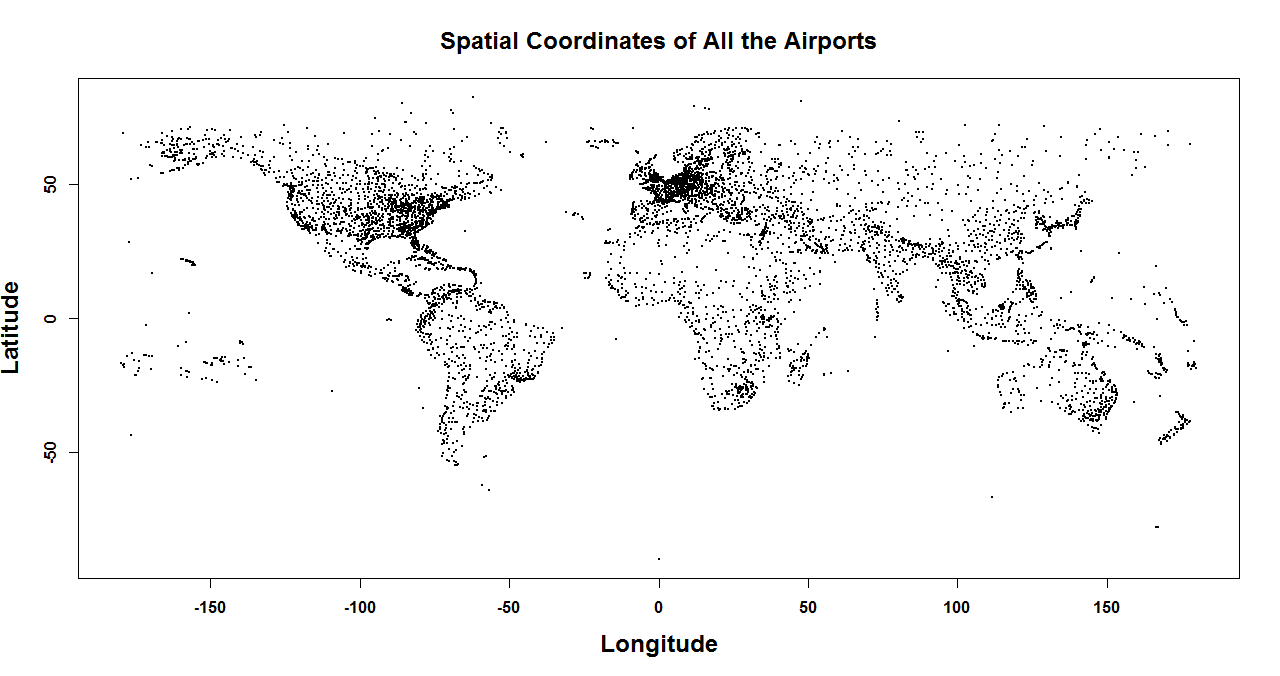
\includegraphics[width=\textwidth, height=\textheight,keepaspectratio]{LonLatMapV2}
	\end{minipage}
	\caption{Passage de paramètres graphiques à la commande \texttt{plot}}
\end{figure}
\label{fig:LonLatMap}

\begin{lstlisting}[caption = Utilisation de la commande \texttt{plot},label=src:plot]
plot(airports$longitude,airports$latitude)
plot(airports$longitude,airports$latitude,cex = 0.1,xlab="Longitude",ylab="Latitude",main="Spatial Coordinates of All the Airports",pch = 20,font = 2,cex.main = 1.5,font.lab = 2,cex.lab = 1.5)
\end{lstlisting}

\vspace{\baselineskip}
Dans le cas où nous aurions plutôt voulu faire la représentation d'une fonction continue, nous pourrions encore une fois utiliser la commande \texttt{plot} en modifiant l'argument \texttt{type}. Bien que cette pratique semble justifiée, elle pourra jouer de mauvais tours aux utilisateurs non-avertis. Comme le montre la \autoref{fig:plotCurve}, dépendamment de l'espacement entre les points calculés, nous pouvous perdre toute l'information sur l'allure réelle de la courbe que nous cherchons à visualiser. \\

Il sera donc préférable d'utiliser la commande \texttt{curve} \cite{Rfunction:curve} pour ce genre de tâche afin de simplifier le code source en ne précisant que les extrêmes de l'étendue sur lequel nous voulons tracer la fonction. Nous pourrons aussi spécifier le nombre de valeurs à calculer dans l'intervalle. \\

\begin{lstlisting}[caption = Utilisation de la commande \texttt{curve},label=src:plotCurve]
fquad <- function(x,a=2,b=3,c=4)
{
  a*x**2+b*x+c
}
fquad(2)
par(mfrow = c(2,2))
plot(x <- seq(-10,10,10),fquad(x,2,3,4),type = "l",ylab = "fquad(x)",xlab = "x",main = "dx = 10")
plot(x <- seq(-10,10,5),fquad(x,2,3,4),type = "l",ylab = "fquad(x)",xlab = "x",main = "dx = 5")
plot(x <- seq(-10,10,2),fquad(x,2,3,4),type = "l",ylab = "fquad(x)",xlab = "x",main = "dx = 2")
plot(x <- seq(-10,10),fquad(x,2,3,4),type = "l",ylab = "fquad(x)",xlab = "x",main = "dx = 1")

par(mfrow = c(1,1))
curve(fquad(x),from = -10,to = 10)
\end{lstlisting}

\addPicture{1}{0.5}{plotCurve}{Tracer une courbe avec la commande \texttt{plot}}{plotCurve}

\addPicture{1}{0.5}{curve}{Tracer une courbe avec la commande \texttt{curve}}{curve}

\vspace{\baselineskip}
Un autre type de graphique fréquemment utilisé dans les analyses statistiques sont les histogrammes. Ces derniers permettent de rapidement avoir une idée globale sur le type de distribution à laquelle nous sommes confrontés. L'argument \texttt{breaks} de la commande \texttt{hist} \cite{Rfunction:hist} est de loin le plus important puisqu'il permettra d'obtenir un visuel plus précis de la situation en réduisant la taille des regroupements effectués. En ne spécifiant qu'un seul nombre à cet argument, nous indiquons à R de diviser les données pour obtenir ce même nombre de groupes de largeur équivalente. Dans le cas où un vecteur de nombre lui serait fourni, R comprendra plutôt qu'il doit regrouper les données en utilisant ces nombres à titre de bornes pour les différents intervalles. Un autre argument bien intéressant est \texttt{freq}. Cet argument booléen contrôlera l'affichage de la hauteur des colonnes de l'histogramme. Le nombre d'observations sera affiché si sa valeur est vraie (valeur par défaut). Autrement, ce sera la probabilité empirique d'observer une valeur dans chacun des regroupements qui sera exhibée. \\

\begin{moreInfo}{\emph{Excel} et les histogrammes}
	Si vous êtes habitués de travailler avec \emph{Excel}, vous avez probablement une mauvaise impression de la valeur ajoutée d'utiliser des histogrammes. Ceci vient du fait qu’ \emph{Excel} travaille plutôt avec des graphiques à bâtons. La différence entre ces deux types de graphique réside dans le fait que les colonnes d'un histogramme possèderont à la fois une largeur et une hauteur, tandis que les diagrammes à bâtons ne possèdent qu'une notion de hauteur et sont plutôt destinés à représenter la distribution d'une variable qualitative. 
\end{moreInfo}

La fonction \texttt{density} \cite{Rfunction:density} est aussi très intéressante d'un côté pratique pour estimer la fonction de densité empirique sous-jacente. Cette fonction possède un argument \texttt{adjust} avec lequel nous contrôlerons le degré de lissage employé. La valeur par défaut de cet argument est 1 et plus sa valeur sera faible, plus nous nous rapprochons de la distribution discrête. Inversement, une valeur supérieure à 1 aura pour effet de lisser davantage la fonction obtenue. \\

Bon nombre des fonctionnalités graphiques de R peuvent être combinées au sein d'un même graphique. Il s'agira d'un comportement natif dans certains cas (les commandes \texttt{points} et \texttt{lines}) ou d'un comportement induit par l'argument \texttt{add} comme c'est possible de le faire avec \texttt{curve}. À titre d'exemple, nous serons en mesure de superposer la fonction de densité renvoyée par \texttt{density} grâce à la commande \texttt{lines}.\\
 
La commande \texttt{abline} \cite{Rfunction:abline} simplifiera grandement l'affichage de fonctions linéaires. L'utilisation de celle-ci pourra se faire de trois manières différentes. La première consiste à spécifier les arguments \texttt{a} et \texttt{b} pour produire la représentation d'une droite d'équation $y = ax + b$. La deuxième permettra plutôt de tracer une droite d'équation $y = h$ en attribuant une valeur à l'argument \texttt{h}. La dernière et non la moindre qui est la plus commode d'entre toutes permet de créer des droites d'équation $x = v$. L'ajout de ce genre de droites permettra de faire ressortir des valeurs d'abscisses ayant une signification particulière dans le cadre de vos analyses. \\

Certaines autres fonctions vous permettront de rajouter de l'information afin de faciliter la lecture de vos graphiques. Parmi ces fonctions, la plus importante sera \texttt{legend} qui comme son nom l'indique, générera une légende au graphique que nous venons de produire. Cette fonction est tout autant paramétrisable que le graphique sous-jacent. Nous pouvons tout de même identifier des arguments plus communs que d'autres. L'argument \texttt{bty} permettra de supprimer l'encadrement de la légende en lui attribuant la valeur "n". Nous préciserons aussi un type de points avec \texttt{pch} ou un type de ligne avec \texttt{lty} sur lesquels nous pourrons affecter la même couleur que la courbe correspondante à l'aide de \texttt{col}. La fonction \texttt{mtext} s'occupera plutôt d'ajouter du texte à des endroits précis sur le graphique pour noter des observations ou ajouter des explications sur des aspects qui nous semblent plus surprenants. \\

L'ensemble des points discutés ci-dessus ont été repris dans le \autoref{src:histAltitude} pour produire la \autoref{fig:histAltitude}. \\

\begin{lstlisting}[caption = {\texttt{hist}, \texttt{density}, \texttt{lines}, \texttt{abline}, \texttt{legend} et \texttt{mtext}},label=src:histAltitude]
Altitude <- as.numeric(paste(airportsCanada$altitude))
hist(Altitude)
hist(Altitude,xlim = c(0,5000))
hist(Altitude,xlim = c(0,5000),breaks = 100)
hist(Altitude,xlim = c(0,5000),breaks = 100,freq = FALSE,col = "gray",border = grey(0.8),font = 2,font.lab = 2)
lines(density(Altitude,adjust = 4),lwd = 2, col = "blue")
lines(density(Altitude,adjust = 1),lwd = 2, col = "purple")
lines(density(Altitude,adjust = 0.25),lwd = 2, col = "red")
altitudeAvg <- round(mean(Altitude),1)
abline(v = altitudeAvg,lwd = 2)
legend(2500,0.0015,legend = c("4","1","0.25"),title = "Density Adjustment \n Factor",col = c("blue","purple","red"),bty = "n",title.col = "black",lty = 1,lwd = 3,y.intersp = 0.5,cex = 1.25)
mtext(paste("Average: \n",altitudeAvg),at = altitudeAvg,cex = 0.75)
\end{lstlisting}

\addPicture{1}{0.5}{histAltitude}{Distribution des altitudes des aéroports canadiens}{histAltitude}

\begin{moreInfo}{Vers l'infini et plus loin encore!}
	Vous aurez compris qu'il ne s'agit que d'un très bref aperçu des capacités graphiques de R. Il existe des structures standards pour générer d'autres types de graphique tels que les diagrammes en pointes de tarte (\texttt{pie}) ou encore les boîtes à moustaches (\texttt{boxplot}). \\
	Certains d'entre vous trouveront peut-être que la génération de graphiques est un processus lent et ardu, mais il s'agit ici du coût à payer pour avoir autant de flexibilité. Ces mêmes personnes seront toutefois heureuses d'apprendre que plusieurs paquetages intègrent des modules de visualisation optimisée pour les objets qui leur sont propres.  Il serait un peu prétentieux de définir et de modifier les options d’affichage par défaut des objets dont l’existence ne dépend aucunement de leur utilisation. \footnote{Rien ne vous empêche de vous-mêmes surdéfinir vos propres fonctions d'affichage pour augmenter votre productivité.} \footnote{Il ne faudra pas oublier de préciser vos options d'affichage avant de partager vos programmes avec des personnes qui n'auraient pas accès à ces dites fonctions.}
\end{moreInfo}